\documentclass[10pt,a4paper]{article}
\usepackage[UTF8,fontset = windows]{ctex}
\setCJKmainfont[BoldFont=黑体,ItalicFont=楷体]{华文中宋}
\usepackage{amssymb,amsmath,amsfonts,amsthm,mathrsfs,dsfont,graphicx}
\usepackage{ifthen,indentfirst,enumerate,color,titletoc}
\usepackage{tikz}
\usepackage{makecell}
\usepackage{longtable}

\usetikzlibrary{arrows,calc,intersections,patterns}
\usepackage[bf,small,indentafter,pagestyles]{titlesec}
\usepackage[top=1in, bottom=1in,left=0.8in,right=0.8in]{geometry}
\renewcommand{\baselinestretch}{1.65}
\newtheorem{defi}{定义~}
\newtheorem{eg}{例~}
\newtheorem{ex}{~}
\newtheorem{rem}{注~}
\newtheorem{thm}{定理~}
\newtheorem{coro}{推论~}
\newtheorem{axiom}{公理~}
\newtheorem{prop}{性质~}
\newcommand{\blank}[1]{\underline{\hbox to #1pt{}}}
\newcommand{\bracket}[1]{(\hbox to #1pt{})}
\newcommand{\onech}[4]{\par\begin{tabular}{p{.9\textwidth}}
A.~#1\\
B.~#2\\
C.~#3\\
D.~#4
\end{tabular}}
\newcommand{\twoch}[4]{\par\begin{tabular}{p{.46\textwidth}p{.46\textwidth}}
A.~#1& B.~#2\\
C.~#3& D.~#4
\end{tabular}}
\newcommand{\vartwoch}[4]{\par\begin{tabular}{p{.46\textwidth}p{.46\textwidth}}
(1)~#1& (2)~#2\\
(3)~#3& (4)~#4
\end{tabular}}
\newcommand{\fourch}[4]{\par\begin{tabular}{p{.23\textwidth}p{.23\textwidth}p{.23\textwidth}p{.23\textwidth}}
A.~#1 &B.~#2& C.~#3& D.~#4
\end{tabular}}
\newcommand{\varfourch}[4]{\par\begin{tabular}{p{.23\textwidth}p{.23\textwidth}p{.23\textwidth}p{.23\textwidth}}
(1)~#1 &(2)~#2& (3)~#3& (4)~#4
\end{tabular}}
\begin{document}
\begin{enumerate}[1.]

\item 函数$f(x)={x^{-\frac 12}}$的定义域是\blank{50}.
\item 集合$A=\{-1, 2m-1\}$, $B=\{m^2\}$, 若$B\subseteq A$, 则实数$m=$\blank{50}.
\item $(1+2x)^5=a_0+a_1x+a_2x^2+a_3x^3+a_4x^4+a_5x^5$, 则$a_3=$\blank{50}
\item 如图, 若正四棱柱$ABCD-A_1B_1C_1D_1$的底面边长为$3$, 高为$4$, 则直线$BD_1$与平面$ABCD$所成角的正切值为\blank{50}.
\begin{center}
    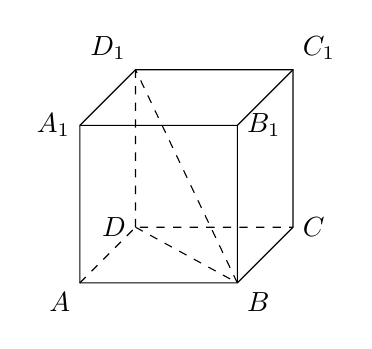
\begin{tikzpicture}
        \draw (0,0) node [below left] {$A$} coordinate (A) --++ (2,0) node [below right] {$B$} coordinate (B) --++ (45:{2/2}) node [right] {$C$} coordinate (C)
        --++ (0,2) node [above right] {$C_1$} coordinate (C1)
        --++ (-2,0) node [above left] {$D_1$} coordinate (D1) --++ (225:{2/2}) node [left] {$A_1$} coordinate (A1) -- cycle;
        \draw (A) ++ (2,2) node [right] {$B_1$} coordinate (B1) -- (B) (B1) --++ (45:{2/2}) (B1) --++ (-2,0);
        \draw [dashed] (A) --++ (45:{2/2}) node [left] {$D$} coordinate (D) --++ (2,0) (D) --++ (0,2);
        \draw [dashed] (D) -- (B) -- (D1);
    \end{tikzpicture}
\end{center}
\item 方程$\lg (x+2)=2\lg x$的解为\blank{50}.
\item 若$\arccos x>\dfrac{\pi}3$, 则$x$的取值范围为\blank{50}.
\item 若函数$f(x)=\sqrt{2x+1}$的反函数为$g(x)$, 则函数$g(x)$的零点为\blank{50}.
\item 已知函数$y=\sin (\omega x-\dfrac{\pi}6)$($\omega >0$)图像的一条对称轴为$x=\dfrac{\pi}6$, 则$\omega$的最小值为\blank{50}.
\item 已知圆锥的底面半径为$1$, 其侧面展开图为一个半圆, 则该圆锥的母线长为\blank{50}.
\item $7$人排成一行, 甲、乙相邻且丙不排两端的排法有\blank{50}种(用数字作答).
\item 设$f(x)$是定义在$\mathbf{R}$上的函数, 且满足$f(1)=0$.若$y=f(x)+a\cdot 2^x$是奇函数, $y=f(x)+3^x$是偶函数, 则$a$的值为\blank{50}.
\item 在$\triangle ABC$中, $b=2,c=1$, $\angle B-\angle C=\dfrac{\pi}2$, 则$\triangle ABC$的周长为\blank{50}.
\item 下列是``$a>b$''的充分不必要条件的是\bracket{20}.
\fourch{$a>b+1$}{$\dfrac ab>1$}{$a^2>b^2$}{$a^3>b^3$}
\item 下列函数中, 既是奇函数, 又是减函数的是\bracket{20}.
\fourch{$y=x^{-1}$}{$y=-\arcsin x$}{$y=\log_2x$}{$y=2^x$}
\item 已知$f(x)=\sin x$, 对任意$x_1 \in[0,\dfrac{\pi}2]$, 都存在$x_2\in [ 0\dfrac{\pi}2]$, 使得$f(x_1)-2f(x_2+\theta)=-1$成立, 则下列$\theta$取值可能的是\bracket{20}.
\fourch{$\dfrac{3\pi}{13}$}{$\dfrac{5\pi}{13}$}{$\dfrac{7\pi}{13}$}{$\dfrac{9\pi}{13}$}
\item 非空集合$A\subseteq \mathbf{R}$, 且满足如下性质:
性质一: 若$a,b\in A$, 则$a+b\in A$;
性质二: 若$a\in A$, 则$-a\in A$, 则称集合$A$为一个``群''. 以下叙述:\\
\textcircled{1} 若$A$为一个``群'', 则$A$必为无限集;
\textcircled{2} 若$A$为一个``群'', 且$a,b\in A$, 则$a-b\in A$;
\textcircled{3} 若$A,B$都是``群'', 则$A\cap B$必定是``群'';
\textcircled{4} 若$A,B$都是``群'', 且$A\cup B\ne A,A\cup B\ne B,$则$A\cup B$必定不是``群''.\\
中, 正确的个数为\bracket{20}.
\fourch{$1$}{$2$}{$3$}{$4$}
\item 如图, 在正三棱柱$ABC-A_1B_1C_1$中, $AA_1=2$, $AB=3$, 点$D$为$BC$的中点.
\begin{center}
    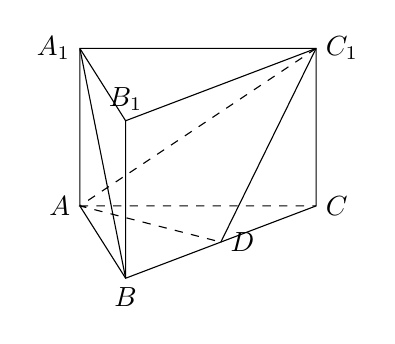
\begin{tikzpicture}
        \draw (0,0) node [left] {$A$} coordinate (A);
        \draw (3,0) node [right] {$C$} coordinate (C);
        \draw (1.5,0) ++ (225:{3/4*sqrt(3)}) node [below] {$B$} coordinate (B);
        \draw (A) ++ (0,2) node [left] {$A_1$} coordinate (A1);
        \draw (B) ++ (0,2) node [above] {$B_1$} coordinate (B1);
        \draw (C) ++ (0,2) node [right] {$C_1$} coordinate (C1);
        \draw (A) -- (B) -- (C) -- (C1) -- (A1) -- (A) (B) -- (B1) -- (A1) (B1) -- (C1);
        \draw ($(B)!0.5!(C)$) node [right] {$D$} coordinate (D);
        \draw (A1) -- (B) (D) -- (C1);
        \draw [dashed] (C1) -- (A) -- (D) (A) -- (C);
    \end{tikzpicture}
\end{center}
(1) 求证: 直线$A_1B$与$C_1D$为异面直线;\\
(2) 求三棱锥$B-AC_1D$的体积.
\item 已知代数式$(\dfrac 2m+\dfrac mx)^n$($m>0$, $x>0$).\\
(1) 当$m=2$, $n=6$时, 求二项展开式中二项式系数最大的项;\\
(2) 若$(\dfrac 2m+\dfrac mx)^{10}=a_0+\dfrac{a_1}x+\dfrac{a_2}{x^2}+\cdots +\dfrac{a_{10}}{x^{10}}$, 且$a_2=180$, 求$a_i$($0\le i \le 10$, $i\in \mathbf{N}$)的最大值.
\item 为实现``碳达峰'', 减少污染, 某化工企业开发了一个废料回收项目. 经测算, 该项目日回收成本$p$(元)与日回收量$x$(吨)($x\in [0,50]$)的函数关系可表示为$p=\begin{cases}20x, & 0\le x\le 30,  \\ x^2+16x-780, & 30<x \le 50,  \end{cases}$ 且每回收$1$吨废料, 转化成其他产品可收入$80$元.\\
(1) 设日纯收益为$y$元, 写出函数$y=f(x)$的解析式(纯收益$=$收入$-$成本);\\
(2) 该公司每日回收废料多少吨时, 获得纯收益最大?
\item 已知函数$f(x)=2^x+\dfrac a{2^x}$, $a$为实常数.\\
(1) 若函数$f(x)$为奇函数, 求$a$的值;\\
(2) 若$x\in [0,1]$时$f(x)$的最小值为$2$, 求$a$的值;\\
(3) 若方程$f(x)=6$有两个不等的实根$x_1,x_2$, 且$|x_1-x_2|\le 1$, 求$a$的取值范围.
\item 若实数$x,y\in [0,2\pi]$, 且满足$\cos (x+y)=\cos x+\cos y$, 则称$x$与$y$是``余弦相关''的.\\
(1) 若$x=\dfrac{\pi}2$, 求出所有与之``余弦相关''的实数$y$;\\
(2) 若存在实数$y$, 与$x$``余弦相关'', 求$x$的取值范围;\\
(3) 若不相等的两个实数$x$与$y$是``余弦相关''的, 求证: 存在实数$z$, 使得$x$与$z$ 为``余弦相关''的, $y$与$z$也为``余弦相关''的.

\end{enumerate}
\end{document}